\documentclass[final,t]{beamer}
\mode<presentation>
{
 \usetheme{I6dv}
%  \usetheme{I6pd2}
}
% additional settings
\setbeamerfont{itemize}{size=\normalsize}
\setbeamerfont{itemize/enumerate body}{size=\normalsize}
\setbeamerfont{itemize/enumerate subbody}{size=\normalsize}

% additional packages
\usepackage{times}
\usepackage{amsmath,amsthm, amssymb, latexsym}
% \usepackage{algpseudocode}
\usepackage{exscale}
\usepackage{color}
%\boldmath
\usepackage{booktabs, array}
%\usepackage{rotating} %sideways environment
\usepackage[english]{babel}
\usepackage[latin1]{inputenc}
\usepackage[orientation=landscape,size=custom,width=200,height=120,scale=1.9]{beamerposter}
\listfiles
\graphicspath{{figures/}}
% Display a grid to help align images
%\beamertemplategridbackground[1cm]

\title{\huge A Gpu Implementation of Von Mises-Fisher Distribution Algorithm for Polymer Conformation Analysis}
\author[Abzhanov et al.]{Aidos Abzhanov, Bakytzhan Kallemov}
\institute[Nazarbayev University, Astana, Kazakhstan]{Center for Energy Research, Nazarbayev University, Astana, Kazakhstan}
\date[Jul. 2012]{Jul., 2012}

% abbreviations
\usepackage{xspace}
\makeatletter
\DeclareRobustCommand\onedot{\futurelet\@let@token\@onedot}
\def\@onedot{\ifx\@let@token.\else.\null\fi\xspace}
\def\eg{{e.g}\onedot} \def\Eg{{E.g}\onedot}
\def\ie{{i.e}\onedot} \def\Ie{{I.e}\onedot}
\def\cf{{c.f}\onedot} \def\Cf{{C.f}\onedot}
\def\etc{{etc}\onedot}
\def\vs{{vs}\onedot}
\def\wrt{w.r.t\onedot}
\def\dof{d.o.f\onedot}
\def\etal{{et al}\onedot}
\makeatother
\def\O{{\mathcal O}}
\def\xv{{\bf x}}
\def\qv{{\bf q}}
\def\zv{{\bf z}}
\def\vv{{\bf v}}
\def\uv{{\bf u}}
\def\cv{{\bf c}}
\def\fv{{\bf f}}
\def\yv{{\bf y}}
\def\Yv{{\bf Y}}
\def\Ib{{\bf I}}
\def\Fv{{\bf F}}
\def\Rv{{\bf R}}
\def\Uv{{\bf U}}
\def\av{{\bf a}}
\def\bv{{\bf b}}
\def\rv{{\bf r}}
\def\Wv{{\bf W}}
\def\Xv{{\bf X}}
\def\Gammab{{\mbox{\boldmath{$\Gamma$}}}}
%%%%%%%%%%%%%%%%%%%%%%%%%%%%%%%%%%%%%%%%%%%%%%%%%%%%%%%%%%%%%%%%%%%%%%%%%%%%%%%%%%%%%%%%%%%%%%%%%%%%%%%%%%%%
%%%%%%%%%%%%%%%%%%%%%%%%%%%%%%%%%%%%%%%%%%%%%%%%%%%%%%%%%%%%%%%%%%%%%%%%%%%%%%%%%%%%%%%%%%%%%%%%%%%%%%%%%%%%
\begin{document}
\begin{frame}{} 
  \begin{columns}[t]
    \begin{column}{.3\linewidth}

      %%%%%%%%%%%%%%%%%%%%%%%%%%%%%%%%%%%%%%%%%%%%%%%%%%%%%%%%%%%%%%%%%%%%%%%%%%%%%%%%%%%%%%%%%%%%%%%%%%%%%%%%%%%%

      \begin{block}{Motivation}
        \begin{itemize}
		\item Multiscale models for polymer
	     \vskip2ex              
         \centerline{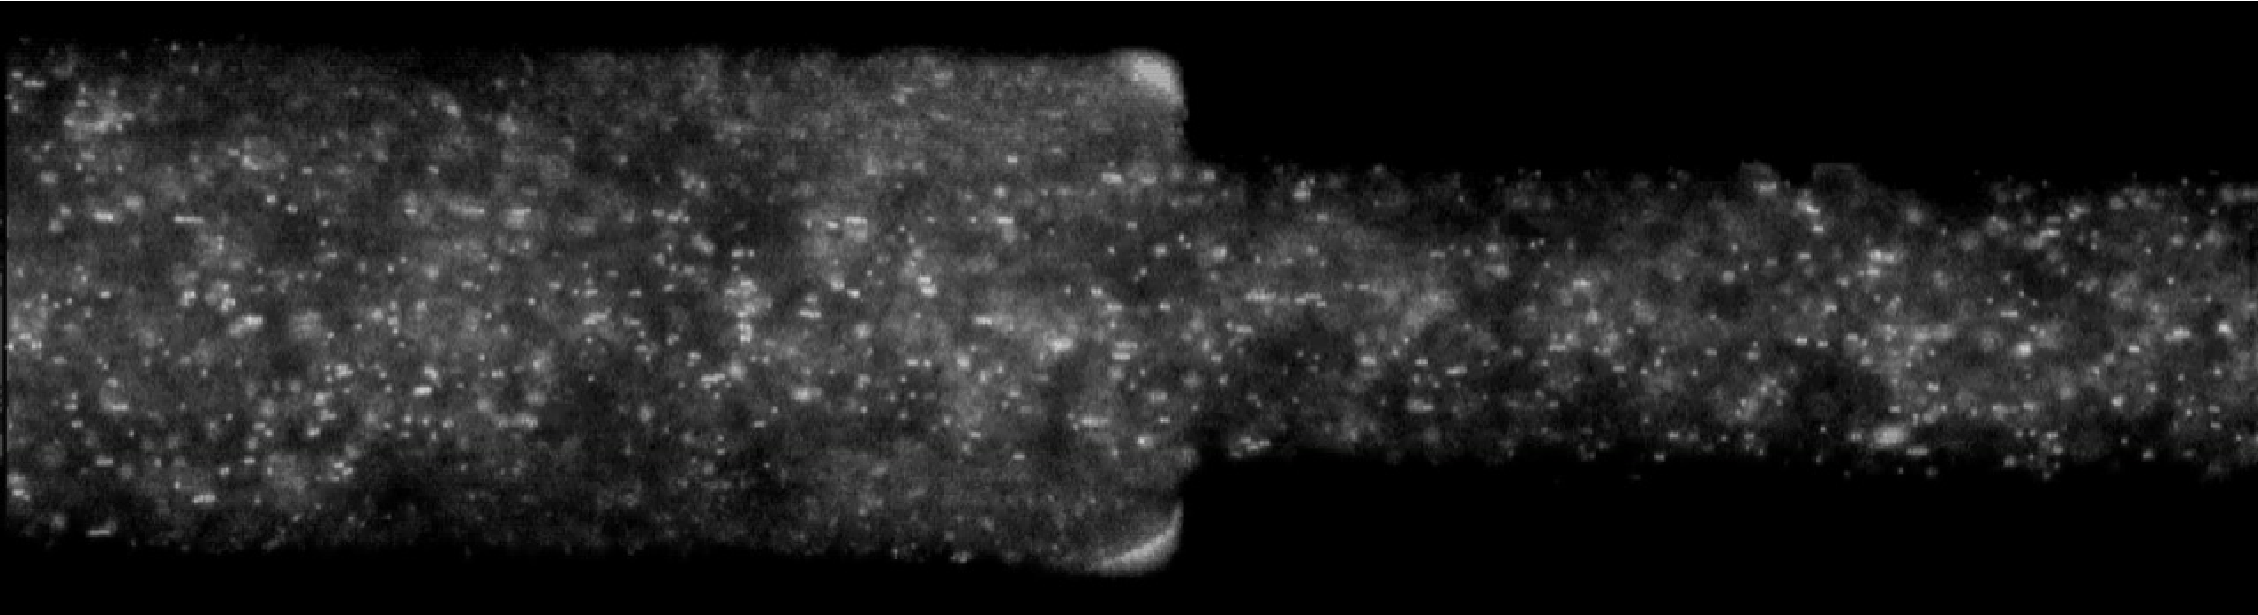
\includegraphics[width=0.8\linewidth]{figures/nonnewtonian}}
		{\bf Advantages:}
        \item generally compare better to experiments than pure macroscopic models
        \item avoid potentially harmful closure operation
        \item more descriptive and universal 
		\\{\bf Disadvantages:}
        \item Highly computationally demanding
        \item no universal approach to the problem
        \end{itemize}
      \end{block}

      %%%%%%%%%%%%%%%%%%%%%%%%%%%%%%%%%%%%%%%%%%%%%%%%%%%%%%%%%%%%%%%%%%%%%%%%%%%%%%%%%%%%%%%%%%%%%%%%%%%%%%%%%%%%
      
      \begin{block}{Kramers bead-rod freely jointed polymer model}
            \begin{itemize}
	       \item Kinetic model of the polymers
	       \item N beads connected by $N-1$ rigid rods. 
           \vskip2ex              
           \centerline{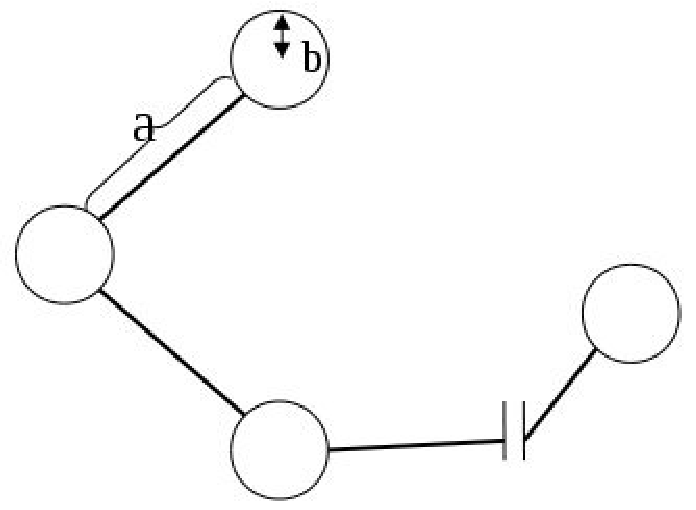
\includegraphics[width=.25\linewidth]{figures/kramer's} \quad \quad \quad
           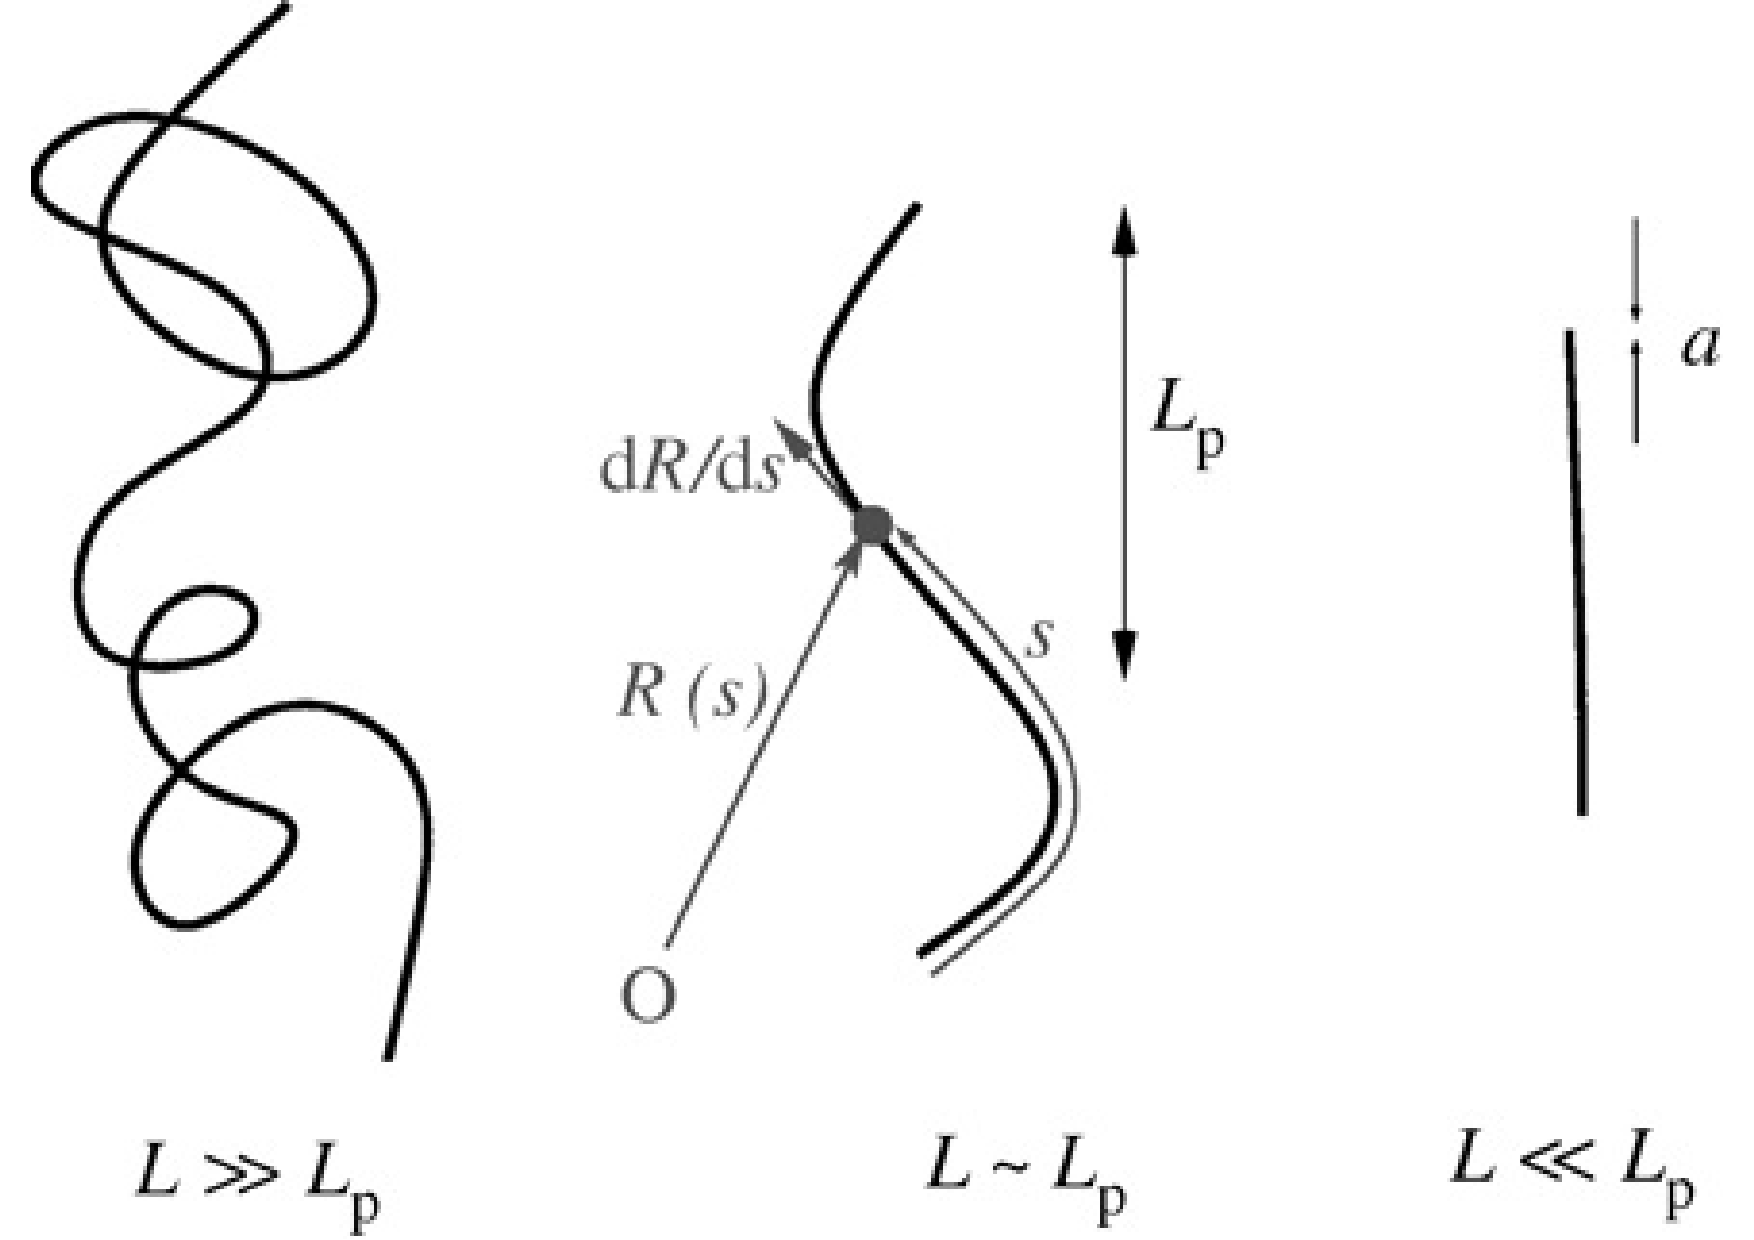
\includegraphics[width=.25\linewidth]{figures/persistence} }
   	       \item For D-dimensional space, total degrees of freedom can be huge \alert{$\O(2\times N\times D\times 10^{23})$}
   	       \item Each of the bead is subjected to constrained Langevin equation
		  \begin{align*}
		    d\xv_\alpha &= \vv_\alpha dt \\
		    d\vv_\alpha &= \gamma(\uv(\xv_\alpha)-\vv_\alpha)dt + \fv_{\rm constraint}dt + \sigma d\Wv
		  \end{align*}

		  Constraint, corresponds to Kuhn length:
			\begin{equation*}
			\theta_{\alpha+1,\alpha}=\frac{1}{2}\left(\| \xv_{\alpha+1}-\xv_\alpha\|^2 -a^2 \right)=0.
			\end{equation*}   	       
        
            \end{itemize}
       \end{block}

      %%%%%%%%%%%%%%%%%%%%%%%%%%%%%%%%%%%%%%%%%%%%%%%%%%%%%%%%%%%%%%%%%%%%%%%%%%%%%%%%%%%%%%%%%%%%%%%%%%%%%%%%%%%%
      \begin{block}{A multiscale framework}
        \begin{columns}[T]
          \begin{column}{.49\linewidth}
    	\centerline{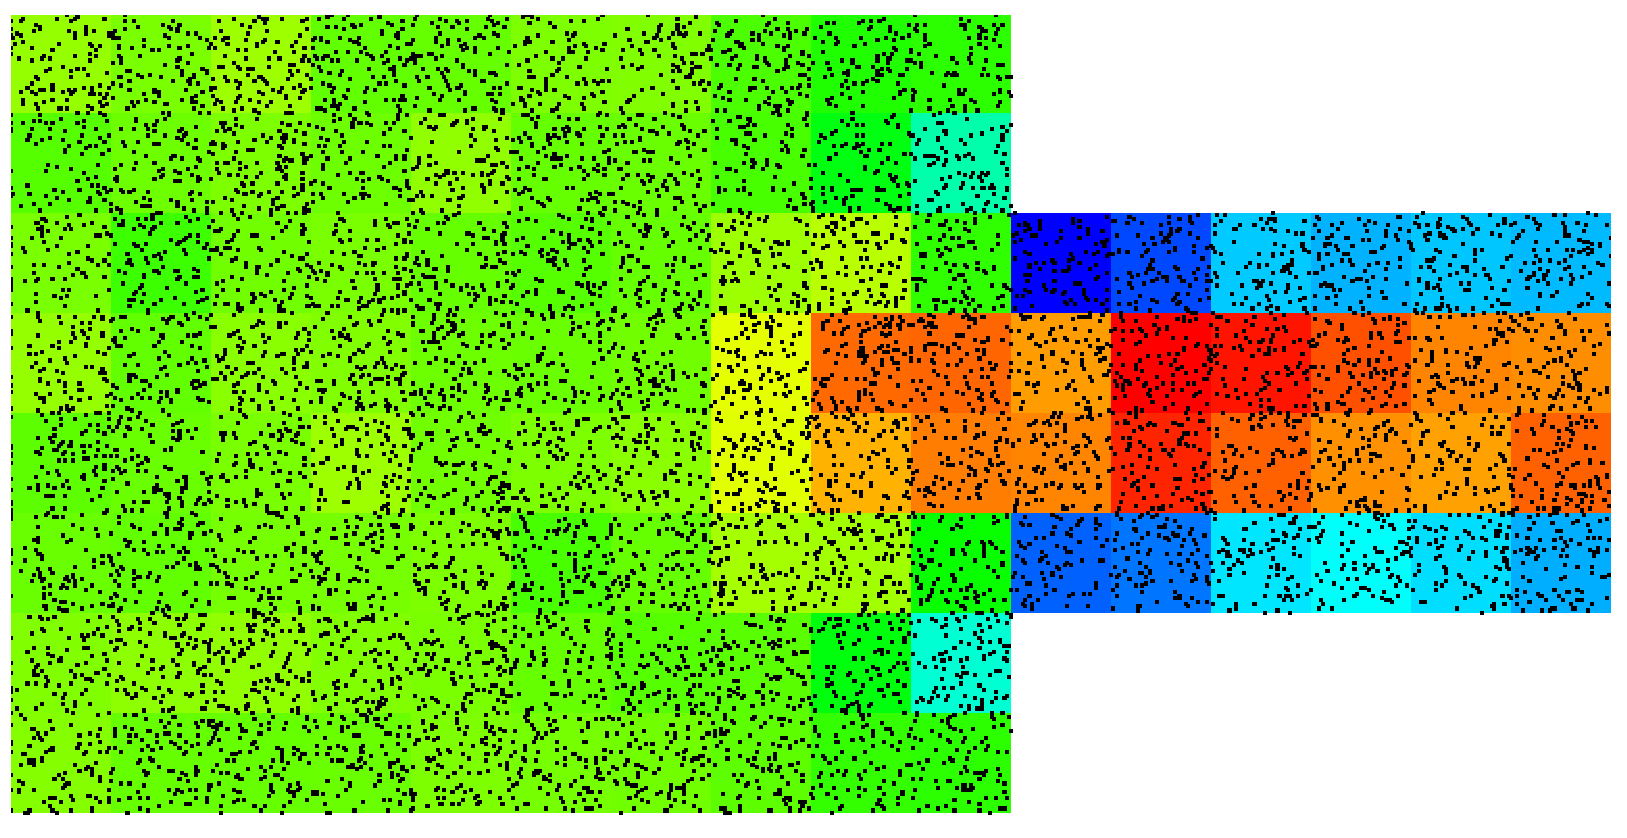
\includegraphics[width=.9 \linewidth]{figures/visit0001}}
    	Lagrangian markers represent a kinetic state, advected with fluid flow
	    \end{column}
	    
       \begin{column}{.49\linewidth}
       Fokker-Planck equation for PDF \cite{Kallemov12}
       \begin{eqnarray*}
		\frac{\partial \Psi}{\partial t} 
			= - \vv \cdot \nabla_\xv \Psi
		     - \nabla_\vv \cdot ( \Fv(\xv,\vv) \Psi) \\
		     + \frac{1}{2} \Gammab_{\alpha \delta}(\xv) \Gammab_{\beta \delta}	
		     		(\xv) \frac{\partial^2 \Psi}{\partial \vv_\alpha \partial \vv_\beta}
		\end{eqnarray*}
		
       \begin{eqnarray*}
		&&\Psi(\qv\vert \xv,t) \rightarrow \\
		&&~~~~~~~\big \{ \qv(t), \vv(t) \rightarrow \qv(t+\Delta t), \vv(t+\Delta t) \big \} \\
		&&~~~~~~~\rightarrow \Psi(\qv\vert \xv+u\Delta t, t+\Delta t )
		\end{eqnarray*}
		
        \end{column}
    
        \end{columns}
	   \end{block}
       
      
    \end{column}
    \begin{column}{.3\linewidth}
      \begin{block}{von Mises-Fisher distribution}
        \vfill
        %\noindent{\textbf{Distribution on Unit sphere}}
        \begin{itemize}
        \item Directional distribution on unit hypersphere in $d$- dimensions, $d \geq 2$
  
	      \begin{align*}
		f(\xv ; \mu, \kappa) = \frac{\kappa^{d/2-1}}{(2\pi)^{d/2}I_{d/2-1}(k)}\exp(\kappa\mu^T\xv)
	      \end{align*}
              \begin{itemize}
              \item $\mu$ - mean direction, $\|\mu\|=1$
              \item $\kappa$ - concentration parameter, $\kappa \geq 0$
              \end{itemize}
        \item for $d=2$ known as von Mises distribution
        \item for $d=3$ known as Fisher distribution
        \end{itemize}
        \vskip1ex
	\begin{columns}[t]
	  \begin{column}{.3\linewidth}
% 	    \raggedleft
	  \small{$ \kappa = 1 $}
	    \includegraphics[width=1.2\linewidth]{figures/kappa=1,N=500}
	    
	  \end{column}
	  \begin{column}{.3\linewidth}
% 	    \raggedleft
	  \small{$ \kappa = 10 $}
	    \includegraphics[width=1.2\linewidth]{figures/kappa=10,N=500}
	    
	  \end{column} 
	  \begin{column}{.3\linewidth}
% 	    \raggedleft
	  \small{$ \kappa = 100 $}
	    \includegraphics[width=1.2\linewidth]{figures/kappa=100,N=500}1
	  \end{column}    
	\end{columns}

%         \vskip1ex
        \noindent{\textbf{Mixture model}}
        \begin{itemize}
        \item Used to characterize distribution in multiple directions
	      \begin{align*}
		f(\xv ; \{\alpha\}, \{\mu\}, \{\kappa\}) = \sum_{h=1}^k \alpha_h f_h(\xv; \mu_h, \kappa_h),
	      \end{align*}
	      where $\alpha_h$ - weight of $h$ direction, $\sum \alpha_h = 0, \alpha_h \geq 0$
        \end{itemize}

        \vskip1ex
        \begin{columns}[T]
          \begin{column}{.4\linewidth}
            \raggedleft
            \includegraphics[width=.9\linewidth]{figures/mixture}
          \end{column}
          \begin{column}{.6\linewidth}
%             \noindent{\hskip1cm\textbf{NVidia Tesla C2075}}\par
            \begin{itemize}
            \item \textcolor{blue}{
	      $\kappa_1 = 20$
	      $\alpha_1 = 0.5$
	      $\mu_1 = (0,1,0)$}
	    \vskip1ex
	    \item \textcolor{orange}{
	      $\kappa_2 = 20$
	      $\alpha_2 = 0.25$
	      $\mu_2 = (-0.66, -0.66, 0.33)$}
	    \vskip1ex
	    \item \textcolor{red}{
	      $\kappa_3 = 30$
	      $\alpha_3 = 0.25$
	      $\mu_3 = (0.707,0,-0.707)$}
            \end{itemize}
          \end{column}
        \end{columns}
%         \begin{columns}[t]
%           \begin{column}{.5\linewidth}
%             \noindent{\hskip1cm\textbf{Features}}\par
%             \begin{itemize}
%             \item \alert{appearance-based image features}: for baseline system
%               \begin{itemize}
%               \item thumb\-nails of video
%               \item give a global descrip
%               \end{itemize}
%             \item \alert{manual features}: 
%               \begin{itemize}
%               \item dominant hand \alert{tracking}: hand position,
%               \end{itemize}
%             \end{itemize}
%           \end{column}
%           \begin{column}{.5\linewidth}
%             \vskip0ex
%             %%%%%%%%%%%%%%%%%%%%%%%%%%%%%%%%%%%%%%%%%%%%%%%%%%%%%%%
%             \centering
%            
%           % \includegraphics[height=0.33\linewidth]{images/u-signlanguage-BOSTON104-videoBank-camera0-001_0_fn000054-0}
%            % \quad\quad
%            % \includegraphics[height=0.33\linewidth]{images/u-signlanguage-BOSTON104-videoBank-camera0-090_0_fn000056-0}
%             \vskip3ex
%            % \includegraphics[height=0.4\linewidth]{images/graphs/trajectory_45_54}
%             \quad
%             %\includegraphics[height=0.4\linewidth]{images/graphs/trajectory_25_34}
%             %%%%%%%%%%%%%%%%%%%%%%%%%%%%%%%%%%%%%%%%%%%%%%%%%%%%%%%
%           \end{column}
%         \end{columns}
        \vspace{-2ex}
      \end{block}

      \begin{block}{Polymer comformation model}
        \begin{columns}[T]
          \begin{column}{.5\linewidth}
%             \noindent{\hskip1cm\textbf{Feature Selection}}\par
            \begin{itemize}
            \item We encode conformation of polymer with mixture of von Mises-Fisher distribution. 
	    \item Instead of storing coordinates of each beads of every polymer in ensemble, we store parameters of corresponding mixture model

            \end{itemize}
          \end{column}
          \begin{column}{.5\linewidth}
      \vspace{-5ex}
%             \raggedleft
            \includegraphics[width=0.7\linewidth]{figures/3_clust_data}
%           \end{column}
%           \begin{column}{.35\linewidth}
%             \raggedleft
      \vspace{-3ex}

            \includegraphics[width=0.7\linewidth]{figures/3_clust_bbold}
          \end{column}
        \end{columns}
      \end{block}

    \end{column}

    %%%%%%%%%%%%%%%%%%%%%%%%%%%%%%%
   
    \begin{column}{.3\linewidth}
    
      \begin{block}{GPU Parallelization}
        \begin{columns}[T]
          \begin{column}{.5\linewidth}
%             \noindent{\hskip1cm\textbf{NVidia Tesla C2075}}\par
            \begin{itemize}
            \item Computation of polymer's conformation is done by EM 
		clusterization algorithm \cite{Banerjee05clusteringon}, \cite{Sra2012} applied to the polymer's rod directions
            \item This is a time-consuming process when computed for ensemble of polymer's realizations.
	    \item We can improve overall performance by moving computations from CPU to GPU
	    
	    \vskip1ex
	    \noindent{\textbf{CUDA Implementation}}\par
	    \item Each polymer realization is computed on a seperate CUDA block
	    \item Shared memory is used to store raelizations's local variables, like data points, $\mu$, $\kappa$, $\alpha$

% 	    \begin{algorithmic}
% 	     \If {$i\geq maxval$}
% 		\State $i\gets 0$
% 	     \EndIf
% 	    \end{algorithmic}
	    \item \texttt{\textbf{kernel}\textless\textless\textless ensemble\_size, polymer\_size\textgreater\textgreater\textgreater (data\_points, mu, kappa, alpha)}


            \end{itemize}
          \end{column}
          \begin{column}{.5\linewidth}
            \raggedleft
            \includegraphics[width=1.0\linewidth]{figures/polymerGrid}
          \end{column}
        \end{columns}

%         \vskip5ex
%         \begin{columns}[T]
%           \begin{column}{.4\linewidth}
%             \noindent{\hskip1cm\textbf{Implementation}}\par
%             \begin{itemize}
%             \item \alert{log-linear combination} of independently
%               trained models
%             \item profit from independent alignments (\eg performing well for long and short words)
%             \item profit from different feature extraction approaches
%             \end{itemize}
%           \end{column}
%           \begin{column}{.6\linewidth}
%             \raggedleft
%             \includegraphics[width=.95\linewidth]{figures/graph1}
%           \end{column}
%         \end{columns}
%         \vspace{-1.5ex}
         \end{block}     
      \begin{block}{Experimental Results}
        %%%%%%%%%%%%%%%%%%%%%%%%%%%%%%%%%%%%%%%%%%%%%%%%%%%%%%%
        \centering
        %\includegraphics[width=0.33\linewidth]{images/pca-ldaw/ldaw}%
        %\includegraphics[width=0.33\linewidth]{images/pca-pcaw/pcaw}%
        %\includegraphics[width=0.33\linewidth]{images/language-model/lm-scale}%
        %%%%%%%%%%%%%%%%%%%%%%%%%%%%%%%%%%%%%%%%%%%%%%%%%%%%%%%

        %%%%%%%%%%%%%%%%%%%%%%%%%%%%%%%%%%%%%%%%%%%%%%%%%%%%%%%
        \begin{table}
          \centering
          %\footnotesize
          %\caption{Baseline results using appearance-based features}
          \begin{tabular}{@{} p{.4\linewidth} r r r @{}}
            \toprule
            Size of ensemble, $(d=3, k=2)$      & CPU (sec)  & GPU (sec) &Acceleration \\
            \midrule
            10					& 0.06            & 0.06    & 1 	\\%\cite{zahedi06bmvc}
            20                                  & 0.13            & 0.08    & 1.6	\\
            30             			& 0.24            & 0.08    & 3 	\\% \cite{dreuw06smvp}
            40                                  & 0.30            & 0.08    & 3.7	\\
            50                                  & 0.36            & 0.08    & 4.5	\\
            60                                  & 0.42            & 0.09    & 4.6	\\
            70                                  & 0.50            & 0.12    & 4.1	\\
%             \addlinespace
%             \addlinespace
%             model-combination                   & 2x100           & 17.9    & 3\\
            \bottomrule
          \end{tabular}
          \label{tab:baseline-results}
        \end{table}
%         \vspace{-1ex}
      \end{block}
      
               
%       \begin{block}{Conclusion}
%         \begin{itemize}
%         \item Conclusion1
%         \item Conclusion2
%         \end{itemize}
%         \vspace{1ex}
% 	 This work is supported by the 055 research program of the MES of the Republic of Kazakhstan
%       \end{block}

      \begin{block}{Reference}
	\small{
	\setbeamertemplate{bibliography item}[text]
	\bibliographystyle{plain}
	\bibliography{poster}
}
%         \vspace{-1ex}

      \end{block}

      \begin{block}{Acknowledgment}
% 	\vspace{-1ex}
	\small{This work was supported by 055 research program from the MES of the Republic of Kazakhstan.}
      \end{block}
%%%%%%%%%%%%%%%%%%%%%%%%%%%%%%%%%%%%%%%%%%%%%%%%%%%%%%%

    \end{column}
  \end{columns}
\end{frame}
\bibliographystyle{plain}
\end{document}


%%%%%%%%%%%%%%%%%%%%%%%%%%%%%%%%%%%%%%%%%%%%%%%%%%%%%%%%%%%%%%%%%%%%%%%%%%%%%%%%%%%%%%%%%%%%%%%%%%%%
%%% Local Variables: 
%%% mode: latex
%%% TeX-PDF-mode: t
%%% End: 